\section{Mathematical Notation}
The ultimate goal of this research is to minimize the execution time of a parallel loop. Here is an example of a hpx for loop. 

\begin{figure*}[h]
	\centering
	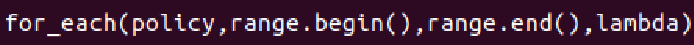
\includegraphics[scale=0.8]{images/for_each_call.pdf}
\end{figure*}

In such loops, a lambda function is applied over a range. The lambda function could be any algorithm like matrix multiplication per example. Each instance of a loop being run will be refered to as an experiment. Each experiment has an unique set of features which will be called $X_i$ for the $i$th experiment. The following 6 features are used:

\begin{itemize}
	\item[1] <Total Number of operations per iteration>
	\item[2] <Number of float operations per iteration>
	\item[3] <Number of comparison operations per iteration>
	\item[4] <Deepest loop level>
	\item[5] <Input size (range)>
	\item[6] <Number of threads>
\end{itemize}

The first 4 features will be referred as static since they only depend on the lambda function internal structure. They are collected at compile time by a ClangTool called loop convert.

The last 2 are called dynamic since they don't depend on the algorithm and are extracted at run-time.

If we assume that the variance in time measurement is small, we can say that time is a function of features and chunk size. If I describe the set of all possible features as $\{X_i\}$ and the set of all possible chunk sizes as $CS$ than we have:

$$t:\{X_i\} \otimes CS \rightarrow \mathbb{R}$$

Our ultimate goal is to find the chunk size that minimizes the execution times for a given set of features. This means that we want to find the function:

\begin{equation}
	f:\{X_i\}\rightarrow cs_i
\end{equation}
 where
\begin{equation}
 cs_i=\underset{cs \in CS}{\arg\min} \, \, t(X_i,cs)
\end{equation}

The  value $cs_i$ is known as optimal chunk size as it minimizes the execution time for experiment $i$. Optimal chunk sizes will be referred to as target values which is the vocabulary used in machine learning for values that we want to predict.

The objective is to use machine-learning algorithms to approximate the function f expressed in (1).
